\chapter{Machine learning approach for true track tagging}
Applying cuts to track features in order to differentiate between improved the ratio of true and false reconstructed tracks, slightly. A more effective
approach in classfying a track as true or false can be achieved with a machine learning algorithm for classification. Unlike one dimensional cuts, a machine learning
algorithm can be implemented to find correlations between the input feature for a more accurate identification of true tracks. The library used for
machine learning is XGBoost, which is explained in the following section. 

\section{XGBoost}
XGBoost \cite{xgboost} is a gradient boosting machine learning algorithm, which primarily uses decision trees as a predictive model for classification and regession analysis.
It is used for supervised learning problems to predict a target variable $y_i$ based on the training data $x_i$ containing multiple features. The model
of XGBoost describes the mathematical structure, which determines the prediction from its input data. A linear model is a common example, where the predictions
are linear combinations of the weighted input features:
\begin{align}
  \hat{y}_i = \sum_j \Theta_j x_{ij}
\end{align}
The coefficents $\Theta$ are indefinite parameters that need to be learned from the training data. Thus, the task of training is in determining the optimal parameters
for the target variable $y_i$ based on our input $x_i$. In order to train a model, an objective function needs to be defined, which measures how well
the model fits the training data. Those functions consist of the training loss function $L(\Theta) $ and the regularization term $\Omega (\Theta)$.
\begin{align}
  \text{obj}(\Theta) = L(\Theta) + \Omega(\Theta)
\end{align}

The training loss function is commonly defined as the mean squared error or logistic loss for logisitc regression problems:
\begin{align}
  &L(\Theta) = \sum_i (y_i - \hat{y}_i)^2 \\
  &L(\Theta) = \sum_i [y_i \ln{(1 + e^{-\hat{y}_i})} + (1 - y_i) \ln{(1 + e^{-\hat{y}_i})}]
\end{align}
The regularization term describes the complexity of a model in order to prevent overfitting.

\section{Decision tree ensemble}
The model used by the XGBoost library is the decision tree ensemble, which consists of a set of classification and regression tress (CART).
A CART assigns a prediction score to each of the leaves in which the input features are classified. The prediction of a single tree is usually not accurate,
therefore the prediction of numerous trees is summed together. This method can be written mathematically as:
\begin{align}
  &\hat{y}_i = \sum_{k=1}^K f_k(x_i)\,, \: f_k \in \mathcal{F} \\
  &\text{obj}(\Theta) = \sum_i^n l(y_i, \hat{y}_i) + \sum_{k=1}^K \Omega(f_k)
\end{align}
Where $K$ is the number of trees, $\mathcal{F}$ the set of all possible CARTs and $f$ a function in $\mathcal{F}$. A decision tree ensemble is shown exemplary in
figure \ref{fig:random_forest}.

\begin{figure}
  \centering
  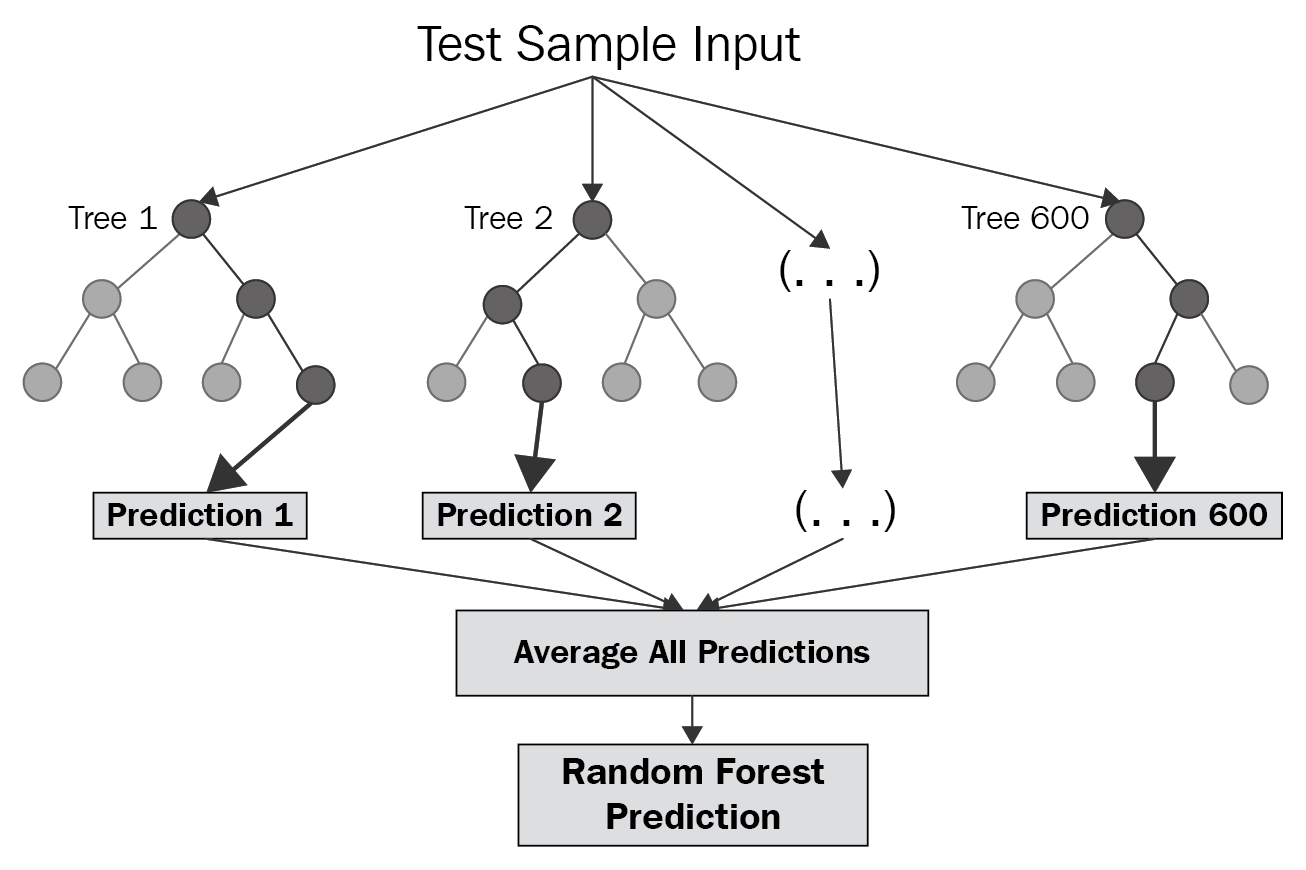
\includegraphics[height=0.6\textwidth]{images/random_forest.png}
  \caption{Representation of a decision tree ensemble \cite{random_forest}.}
  \label{fig:random_forest}
\end{figure}

\section{Boosted trees}
The model used for boosted trees and a random forest is both the tree ensembles with the only difference being the training method. Optimizing the objective functions for
boosted trees is achieved by additive training. This means that everything learned is fixed and only one new tree per step $t$ is added. This can be written
down as follows:
\begin{align}
  \hat{y}_i^{(t)} = \sum_{k=1}^t f_k(x_i) = \hat{y}_i + f_t(x_i)
\end{align}

The tree added in each step is supposed to optimize our objective. For a mean squared error loss function, the objective at step $t$ can be written as:
\begin{align}
  \text{obj}^{(t)} &= \sum_{i=1}^n \left[g_i f_t(x_i)] + \frac{1}{2}h_i f_t^2(x_i)\right] + \Omega(f_t)  \\
  g_i &= \partial_{\hat{y}_i^{(t-1)}} l(y_i, \hat{y}_i^{(t-1)}) \\
  h_i &= \partial^2_{\hat{y}_i^{(t-1)}} l(y_i, \hat{y}_i^{(t-1)})
\end{align}

The value of the objective function only depends on $g_i$ and $h_i$, giving XGBoost the advantage of using custom loss fnctions including logistic regression.

However, the regularization term still needs to be defined. One definition that works well in practice and thus used by XGBoost is:
\begin{align}
  \Omega (f) = \gamma T + \frac{1}{2}\lambda \sum_{j=1}^T \omega_j^2
\end{align}
Here, $\omega_{q(x)}$ is the vector of scores on leaves, $q$ is a function that assigns each data point to the corresponding leave and $T$ is the number of leaves.
